\documentclass{standalone}

\usepackage{circuitikz}

\begin{document}

% INT_AY21_L30_Fig01_Series_parallel.png

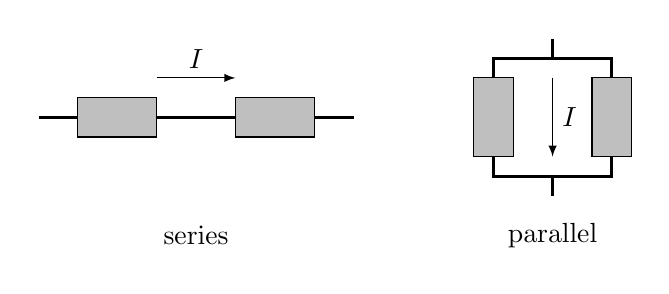
\begin{tikzpicture}[> = latex]
\matrix[column sep = 1.5 cm]{

	% Circuit elements
	
	\begin{scope}[gray!50, draw = black]
	
		\filldraw (-1.5, -0.25) rectangle (-0.5, 0.25);
		\filldraw (0.5, -0.25) rectangle (1.5, 0.25);
	
	\end{scope}
	
	% Wires
	
	\begin{scope}[very thick]
	
		\draw (-2, 0) -- (-1.5, 0);
		\draw (-0.5, 0) -- (0.5, 0);
		\draw (1.5, 0) -- (2, 0);
	
	\end{scope}
	
	% Current flow
	
	\draw [->] (-0.5, 0.5) -- node [above] {$I$} (0.5, 0.5);
	
	% Label
	
	\node at (0, -1.5) {series};

&

	% Circuit elements
	
	\begin{scope}[gray!50, draw = black]

		\filldraw (-1, -0.5) rectangle (-0.5, 0.5);
		\filldraw (1, -0.5) rectangle (0.5, 0.5);
	
	\end{scope}
	
	% Wires
	
	\begin{scope}[very thick]
		
		\draw (0, 0.75) -- (0, 1);
		\draw (-0.75, 0.5) -- (-0.75, 0.75) -- (0.75, 0.75) -- (0.75, 0.5);
		\draw (-0.75, -0.5) -- (-0.75, -0.75) -- (0.75, -0.75) -- (0.75, -0.5);
		\draw (0, -0.75) -- (0, -1);
	
	\end{scope}
	
	% Current flow
	
	\draw [->] (0, 0.5) -- node [right] {$I$} (0, -0.5);
	
	% Label
	
	\node at (0, -1.5) {parallel};

\\	
};

\end{tikzpicture}

\end{document}